\documentclass[a4paper, 12pt]{article}
\usepackage[T2A,T1]{fontenc}
\usepackage[utf8]{inputenc}
\usepackage[english, russian]{babel}
\usepackage{graphicx}
\usepackage[hcentering, bindingoffset = 10mm, right = 13 mm, left = 13 mm, top=20mm, bottom = 20 mm]{geometry}
\usepackage{lipsum}
\usepackage{amsmath, amstext}
\usepackage{siunitx}
\usepackage{subcaption}
\usepackage{wrapfig}
\usepackage{mathrsfs}
\usepackage{adjustbox}
\usepackage{enumerate, indentfirst, float}
\usepackage{capt-of, svg}
\usepackage{icomma}
\usepackage{xcolor}
\usepackage{ctable}
\usepackage{multirow}
\usepackage{amssymb}
\usepackage[version=4]{mhchem}
\usepackage{expl3}
\usepackage{calc}
\usepackage{amsmath}

\newenvironment{bottompar}{\par\vspace*{\fill}}{\clearpage}
 
\begin{document}
\begin{titlepage}

\newcommand{\HRule}{\rule{\linewidth}{0.5mm}} % Defines a new command for the horizontal lines, change thickness here

\center % Center everything on the page
 
%----------------------------------------------------------------------------------------
%	HEADING SECTIONS
%----------------------------------------------------------------------------------------

\textsc{\LARGE Московский Физико-Технический Институт}\\[1,5cm] % Name of your university/college
\textsc{\Large Департамент молекулярной и биологической физики}\\[2cm] % Major heading such as course name
\textsc{\large Лабораторная работа}\\[0.5cm] % Minor heading such as course title

%----------------------------------------------------------------------------------------
%	TITLE SECTION
%----------------------------------------------------------------------------------------

\HRule
\\[0.4cm]
{ \huge \bfseries Активность. Коэффициент активности. pH-метрия}
\\[0.2cm] % Title of your document
\HRule
\\[1.5cm]


 
%----------------------------------------------------------------------------------------
%	AUTHOR SECTION
%----------------------------------------------------------------------------------------
\begin{minipage}{0.4\textwidth}
	\begin{flushleft}		
	\end{flushleft}
\end{minipage}
~
\begin{minipage}{0.4\textwidth}
	\begin{flushright} \large
		\emph{Авторы:}\\
		Светлана \textsc{Фролова} \\
		6113 группа \\
		Анатолий \textsc{Киселёв} \\
		6113 группа
	\end{flushright}
\end{minipage}


\begin{bottompar}
	\begin{center}
		
\includegraphics[width = 80 mm]{logo.jpg}
	\end{center}
	{\large \today}

\end{bottompar}
\vfill % Fill the rest of the page with whitespace

\end{titlepage}

\newpage
\section{Цели работы}
	\begin{enumerate}
	
		\item 
		Знакомство с потенциометрическими методами определения среднеионных коэффициентов активности электролитов и измерения pH растворов;   
		\item 
		Исследование зависимости среднеионного коэффициента активности электролита от его концентрации;   
		\item 
		Исследование влияния ионной силы раствора на растворимость солей;
		\item
		Приобретение практических навыков измерения pH, оценка величины катионной ошибки стеклянного электрода.   
	\end{enumerate}
	
\section{Теоретическая часть}
Химический потенциал компонента реального раствора: 
\[\mu_i(T, p) = \mu_i^0(T, p)+RT\cdot \ln{a_i},\]
где $\mu_i^0(T, p) = \mu_i(T, p_0, a_i = 1)$ - стандартный химический потенциал $i$-ого компонента при температуре $T$ и давлении $p_0 = 105\text{Па}.$ Путём нехитрых преобразований получаем первое выражение для активности:
\begin{equation} \label{act}
a_i = \exp{\left(\frac{\mu_i-\mu_i^0}{RT}\right)}
\end{equation}
Из формулы \ref{act} видно, что активность - сугубо термодинамическая величина, отражающая вклад компонента в свободную энергию Гиббса раствора: 
\[G(T, p) = \sum_{i=1}^n {\nu_i \mu_i}.\] 
Однако размерность и величина активности зависит от используемого способа выражения концентрации - если $a_x$ (активность при выражении концентрации как мольной доли) величина безразмерная, то $a_c$ и $a_m$ (для молярности и моляльности соответственно) - размерные величины, выражаются в моль/л и моль/кг. В
нашей работе концентрация выражается в шкале молярности, соответственно справедлива формула: 
\[\mu_i(T, p) = \mu_{c,i}^0(T, p) + RT \cdot \ln{a_{c,i}}.\]
Индекс $c$ для краткости будем опускать. Активность можно
представить в виде произведения концентрации $c_i$ на коэффициент активности $\gamma_i$:
\begin{equation}
a_i = c_i \cdot \gamma_i
\end{equation}
Ионная сила раствора $I$ - величина, измеряющаяся в единицах концентрации [моль/л] и равная: 
\[I = \frac{1}{2}\sum_i {c_i \cdot z_i^2}.\]
Теория Дебая - Хюккеля позволяет представить коэффициент активности $\gamma_i$ в виде
разности энергии иона типа $i$ в реальном растворе ионной силы $I$ и в предельном случае, когда
ионы вокруг него отсутствуют: 
\[RT \cdot \ln{\gamma_i} = N_A \cdot \bigtriangleup U = N_A(U_I - U_{I=0}).\]
Распределение потенциала
на основе уравнения Пуассона: 
\[\Delta \varphi = - \frac{\rho}{\varepsilon\varepsilon_0} .\]
Плотность заряда на основе распределения Больцмана:
\[\rho(r) =\sum_i{e z_i n_i(r)} = \sum_i{e z_i n_i^0\cdot \exp{\left(\frac{-ez_i\varphi(r)}
{kT}\right)}} .\] 
В первом приближении ионы считаются точечными
и $ez_i\varphi (r) \ll kT$. Распределение электрического потенциала вокруг некоторого иона в приближении
теории Дебая-Хюккеля: 
\[\varphi_i(r) =\frac{ez_i}{4 \pi \varepsilon \varepsilon_0} \exp{-\varkappa   r}.\]
Происходит экранировка собственного потенциала иона:
\[\varphi_i(r) = \frac{z_ie}{4\pi \varepsilon \varepsilon_0},\]
где $\varkappa  $ - постоянная экранирования: 
\[\varkappa   = \frac{1}{r_D} = \sqrt{\frac{e^2}{\varepsilon \varepsilon_0 kT} \left( \sum_i n_i^0z_i^2\right) }.\]
Таким образом, добавка
к энергии, обусловленная взаимодействием иона с его ионной атмосферой: 
\[\Delta U = ez_i\left(\frac{\varphi-\varphi_i}{2}\right)_{r\rightarrow 0} = -\frac{e^2z_i^2\varkappa  }
{8\pi\varepsilon\varepsilon_0}.\]
Из описанного приближения вытекает предельный закон Дебая-Хюккеля:
\begin{equation}
\lg{\gamma_i}=-z_i^2h\sqrt{I}
\end{equation}
Измерить активность ионов одного типа не удается, так как нельзя создать систему с ионами только
одного типа - она не будет электронейтральной. Измерению поддаются только активности ионов при наличии ионов, компенсирующих их заряд. Для такой системы принято говорить о среднеионном
коэффициенте активности: 
\[\gamma_\pm^{\nu_++\nu_-}= \gamma_+^{\nu_+}\gamma_-^{\nu_-}.\]
Таким образом, в первом приближении теории Дебая-
Хюккеля $(I<0.01M)$: 
\[\lg{\gamma_\pm} = -0.51\vert z_+z_-\vert \sqrt{I}.\] 
Во втором приближении $(I<0.1M)$ учитывается то, что центры ионов не могут приближаться друг к другу на расстояние меньше некоторого a: \[\lg{\gamma_\pm} = -0.51\vert z_+z_-\vert\left( \frac{\sqrt{I}}{1+\sqrt{I}}\right).\]
Третье приближение рассматривает более широкий диапозон концентраций: 
\[\lg{\gamma_\pm} = -0.51\vert z_+z_-\vert \left(\frac{\sqrt{I}}{1+\sqrt{I}}-0.2I\right).\]
Величина водородного потенциала $pH$ определяется активностью ионов
водорода в растворе:
\begin{equation}
pH = -\lg{a_{H^+}}
\end{equation}
Разность потенциалов между электродами: 
\[E_X = E_0 - b \cdot pH.\]
Коэффициент активности ионов водорода: 
\[\gamma_{H^+} = \frac{10^{-pH}}{c_{H^+}}
= \frac{10^{\frac{(E^{st}-E_X)}{b^{st}}}}{c_{H^+}},\]
где $E_0^{st}$ и $b^{st}$ - величины, найденные при градуировке. Электрод - система, состоящая из нескольких фаз, на границе которых направленное движение электронов
меняется на направленное движение ионов или наоборот. Индикаторный электрод - электрод, чей
потенциал меняется в зависимости от $pH$ исследуемого раствора. Ключевым элементом обоих электродов является хлорсеребрянный электрод. Полуреакция для него:
\begin{equation}
AgCl_{(s)} + e^- \rightleftarrows  Ag_s^0 + Cl_{sol}^-
\end{equation}
Потенциал такого электрода: 
\[\varphi = \varphi^0 + \frac{RT}{F} \ln{a_{Ag^+}} =\varphi^0 + \frac{RT}{F} \ln{a_{AgCl}} - \frac{RT}{F} \ln{a_{Cl^-}} = \varphi_2^0-\frac{RT}{F} \ln{a_{Cl^-}}.\]
В качестве индикаторного электрода для ионов $H^+$ используется стеклянный электрод. Схема такой
части электрохимической цепи: 
\[Ag\vert AgCl, 0.1M HCl\vert \text{стекло}\vert \text{раствор}.\] 
Потенциал стеклянного электрода: 
\[\varphi = \varphi_1^0+\frac{RT}{F} \ln{(a_{H^+} + Ka_{Na^+})}.\] 
Приближенное выражение для водородного потенциала: 
\[E_X \backsimeq E' - \frac{RT\ln{10}}{F} pH_X.\] 
При объединении электродов в цепь может получиться так, что между собой контактируют растворы полуячеек различного качественного и/или количественного состава. Происходит разделение положительных и отрицательных зарядов на атомном расстоянии, что по законам
электростатики приводит к возникновению скачка электрического потенциала, называемого диффузионным потенциалом.

\newpage
\section{Обработка результатов}
\subsection{Исследование влияние ионной силы на растворимость труднорастворимой соли}
В ходе опыта измерили значение электропроводности для ряда растворов, данные представлены в таблице 1:


\begin{enumerate}
\item Оценим вклад электропроводности СaSO4 в присутствии солей хлорида калия и сульфата натрия:

\[x_{\ce{CaSO_4}} = x - x_{\ce{KCl}} - x_{\ce{H2O}}\]

В присутствии \ce{KCl} : 2156,56 мкСм/cм

В присутствии \ce{Na2SO4}: 1702,56 мкСм/cм

\item Найдем концентрации ионов \ce{Ca^{2+}} \ce{SO4^{2-}} в присутствие и в отсутствие других солей:

Учитывая, что $\frac{1}{2} \lambda_{\ce{Ca^2+}} = 59.5  \frac{\text{Cм}\cdot\text{см}^2}{\text{моль}} \frac{1}{2} \lambda_{\ce{SO4^2-}} = 79.8 \frac{\text{Cм}\cdot \text{см}^2}{\text{моль}}$:

\[C\cdot \lambda = x\]

Тогда : 
\[C = \frac{x}{\left( \frac{1}{2} \lambda_{\ce{Ca^2+}} +\frac{1}{2} \lambda_{\ce{SO4^2-}} \right)}\]

Чтобы рассчитать произведение растворимости для начала нужно найти коэффициенты активности по формуле:

\[\lg{\gamma_i} = -0,51 z_i^2\cdot \sqrt{I}\]
\[\gamma_{\ce{H2O}}= 0.299;\]
\[\gamma_{\ce{KCl}}= 0.267;\]
\[\gamma_{\ce{Na2SO4}}=0.28\]

\[\text{ПР}_{\ce{CaSo4}}=2.2\cdot 10^{-5}; 1.71\cdot 10^{-5}; 1.17\cdot 10^{-5}\]

Сульфат натрия понижает значение ПР и ухудшает растворимость сульфата кальция в воде.

\end{enumerate}
\newpage
\subsection{Калибровка pH-метра}


\begin{figure}[h]
	\centering
	\caption{}	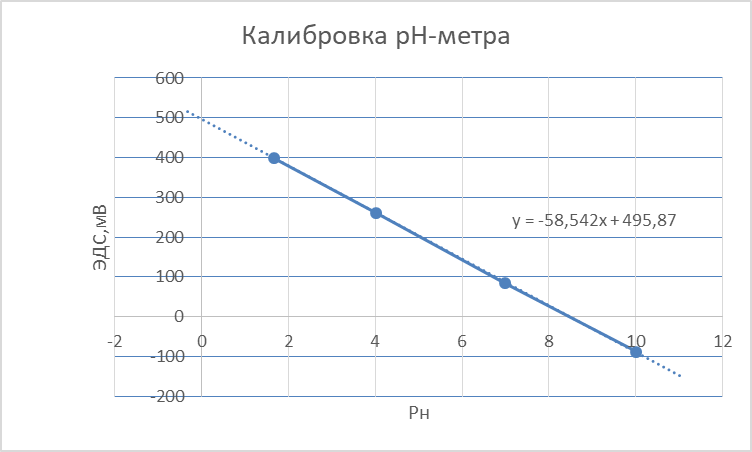
\includegraphics[width=1\textwidth]{image001.png}
\end{figure}
\newpage
\subsection{Определение коэффициента активности и среднеионного коэффициента активности}

\begin{enumerate}
\item
По результатам измерений построим графики зависимости ЭДС от pH для двух электродов: комбинированного стеклянного и хлорсеребряного и электрода сравнения\\

\begin{figure}[h!]
	\centering
	\caption{}
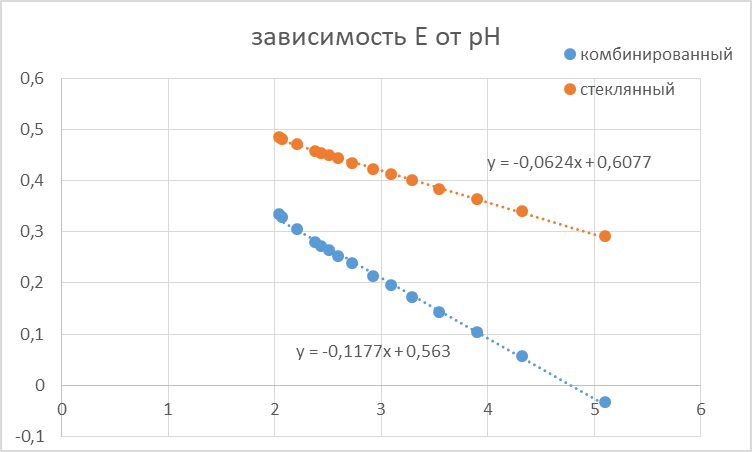
\includegraphics[width=0.8\textwidth]{image003.png}
\end{figure}
Угловые коэффициенты графиков: 62,4 мВ и 117,7 мВ

\item
Построим график зависимости $E - \frac{2RT}{F\cdot \ln{10}\cdot \lg{C_{HCl}}}$ от корня из ионнной силы $\sqrt{J}$\\

\begin{figure}[h!]
	\centering
	\caption{}
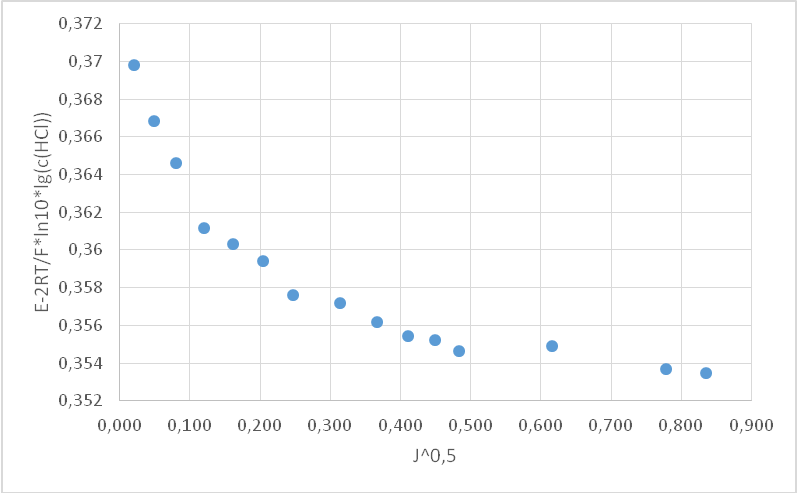
\includegraphics[width=0.8\textwidth]{image005.png}
\end{figure}
\end{enumerate}
Линейной экстраполяцией графика находим $E_0 = 364.4 \text{мВ}$

Построим график зависимости

$Y = E - 0.1183\lg{C_{HCl}} + 0.059 \frac{\sqrt{C_{HCl}}}{\sqrt{1+ C_{HCl}}}$ от $C_{HCl}$\\

\begin{figure}[h!]
	\centering
	\caption{}
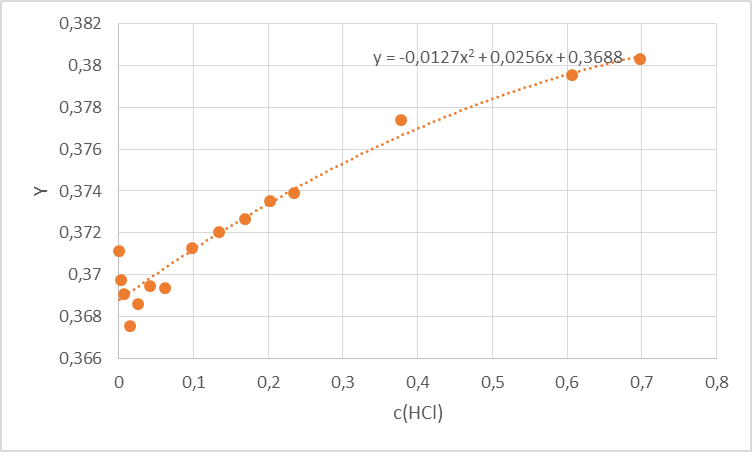
\includegraphics[width=0.8\textwidth]{image007.png}
\end{figure}
\subsection{Исследование водородной функции стеклянного электрода}


\begin{figure}[h!]
	\centering
	\caption{}
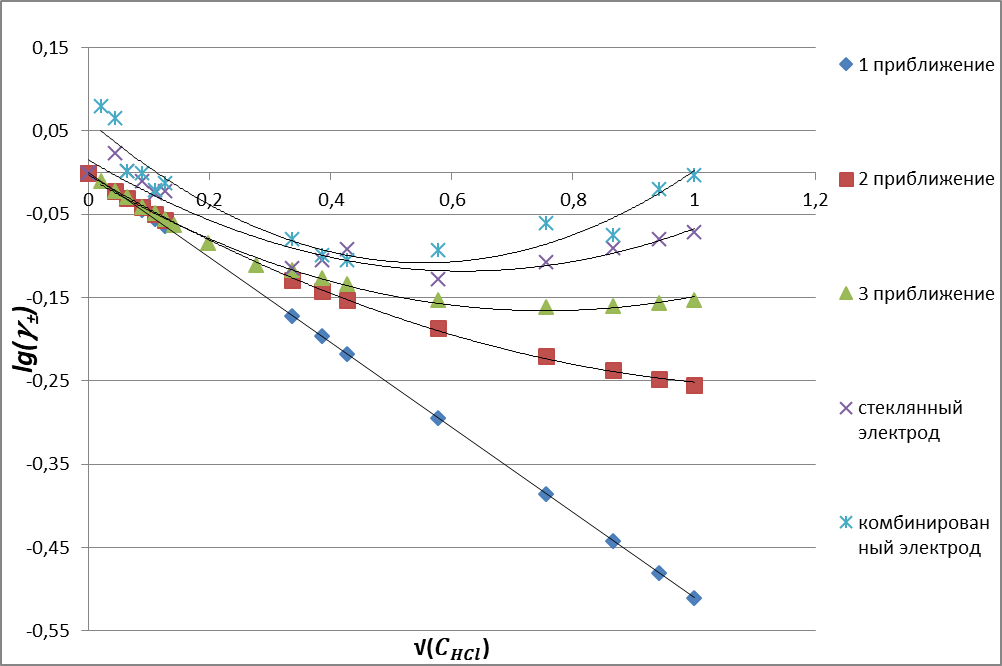
\includegraphics[width=0.8\textwidth]{image013.png}
\end{figure}
\newpage

\begin{figure}[t]
	\centering
	\caption{}
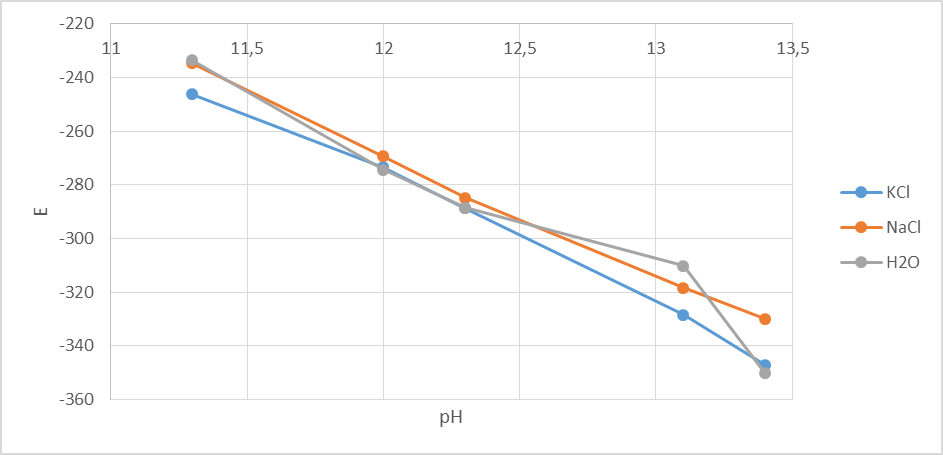
\includegraphics[width=1\textwidth]{image015.png}
\end{figure}

\begin{figure}[h!]
	\centering
	\caption{}
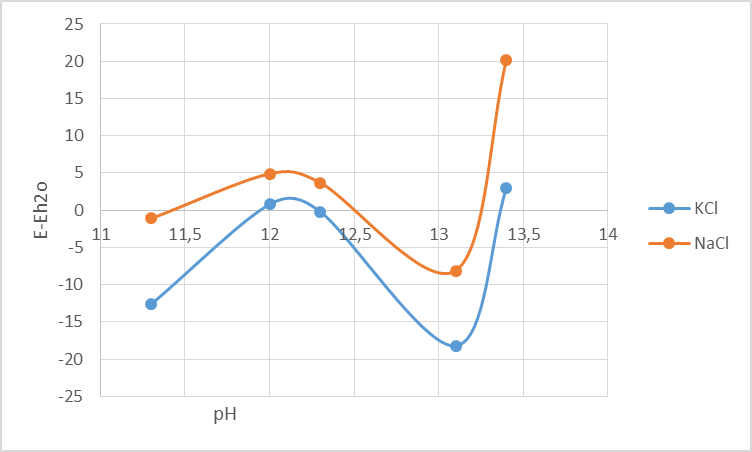
\includegraphics[width=1\textwidth]{image017.png}
\end{figure}

\newpage
\section{Вывод}
В ходе работы мы ознакомились с потенциометрическими методами определения среднеионных коэффициентов активности электролитов и измерения pH растворов, исследовали зависимости среднеионного коэффициента активности электролита от его концентрации, а также влияние ионной силы раствора на растворимость солей.
\end{document}